\subsection{Completed results}

\begin{center}\small
\begin{tabular}{lrrrr}
\toprule
Policy & Astro., $b=1$ & Astro., $b=5$ & Football, $b=1$ & Football, $b=5$ \\
\midrule
Static ranking & 0.0603 & 0.0726 & 0.1364 & 0.1783 \\
Last value & 0.0623 & 0.0726 & 0.1460 & 0.1803 \\
Round robin & 1.2396 & 0.7498 & 1.5487 & 0.9725 \\
IID UCB & 0.0603 & 0.0730 & 0.1364 & 0.1808 \\
IID TS & 0.0603 & 0.0721 & 0.1364 & 0.1811 \\
Window UCB & 0.0603 & 0.1119 & 0.6193 & 0.2994 \\
AR greedy & 0.0625 & 0.0800 & 0.1453 & 0.1296 \\
AR predictive UCB & 0.0650 & 0.0714 & 0.1803 & 0.1437 \\
AR predictive TS & 0.0823 & 0.0817 & 0.5313 & 0.2336 \\
Joint greedy & 0.0603 & 0.0670 & 0.1408 & 0.1417 \\
Joint state UCB & 0.0603 & 0.0528 & 0.1507 & 0.1315 \\
Joint state TS & 0.0797 & 0.0811 & 0.4872 & 0.2515 \\
Joint predictive UCB & 0.0603 & 0.0539 & 0.1647 & 0.1362 \\
Joint predictive TS & 0.0628 & 0.0663 & 0.3911 & 0.2053 \\
Rewired predictive TS & 0.0628 & 0.0653 & 0.3871 & 0.2059 \\
Graph-free factor/shrink TS & 0.0712 & 0.0716 & 0.4302 & 0.2107 \\
Graph-free shrink/factor TS & 0.0712 & 0.0716 & 0.4302 & 0.2107 \\
\bottomrule
\end{tabular}\end{center}


The study completed 352 runs and 63,712 daily decisions in 197.9 seconds, with 166.8 MB peak process memory. AR(7) filter covariances contain 192 state coordinates; AR(20) contains 504. End-to-end experiment time includes development, fitting, initialization, both batch budgets and the sensitivity runs.

With five readings per day, joint predictable-state UCB reduces regret relative to its matched temporal-only rule by 24.5\% in astronomy and 5.2\% in football. Against static ranking the football reduction is 23.6\%. Temporal-only greedy attains .1296 on football and remains slightly better than the corresponding joint UCB rules; there is no uniform joint-policy winner.

With one reading per day, static ranking and IID rules are very strong. The dominant article is already well identified by the full training history. Joint predictable-state TS improves on full-state TS but still loses substantially to static or greedy policies in the football panel. Exploration of learnable uncertainty can be unnecessary at this mature-catalog budget; removing fresh noise is useful but insufficient to ensure good finite-horizon allocation.

The real and rewired hyperlink covariances give essentially the same predictive-sampling regret. Astronomy one-arm policies coincide to the reported precision; five-arm differences are small, and football results are similarly close. The experiment demonstrates effects of correlated covariance and temporal modelling, but does not establish added value of the actual historical hyperlink topology. Common-factor and empirical-covariance controls select identical fits because their target families overlap here.

The dense AR(20) sensitivity is stable without coefficient rescaling. Astronomy five-arm joint predictive UCB regrets .0522 versus .0655 for the AR-only rule, a 20.4\% reduction. Football gives .1320 versus .1356. Higher order is feasible on this laptop, but benefits depend on the instance and metric.

\begin{figure}[t]\centering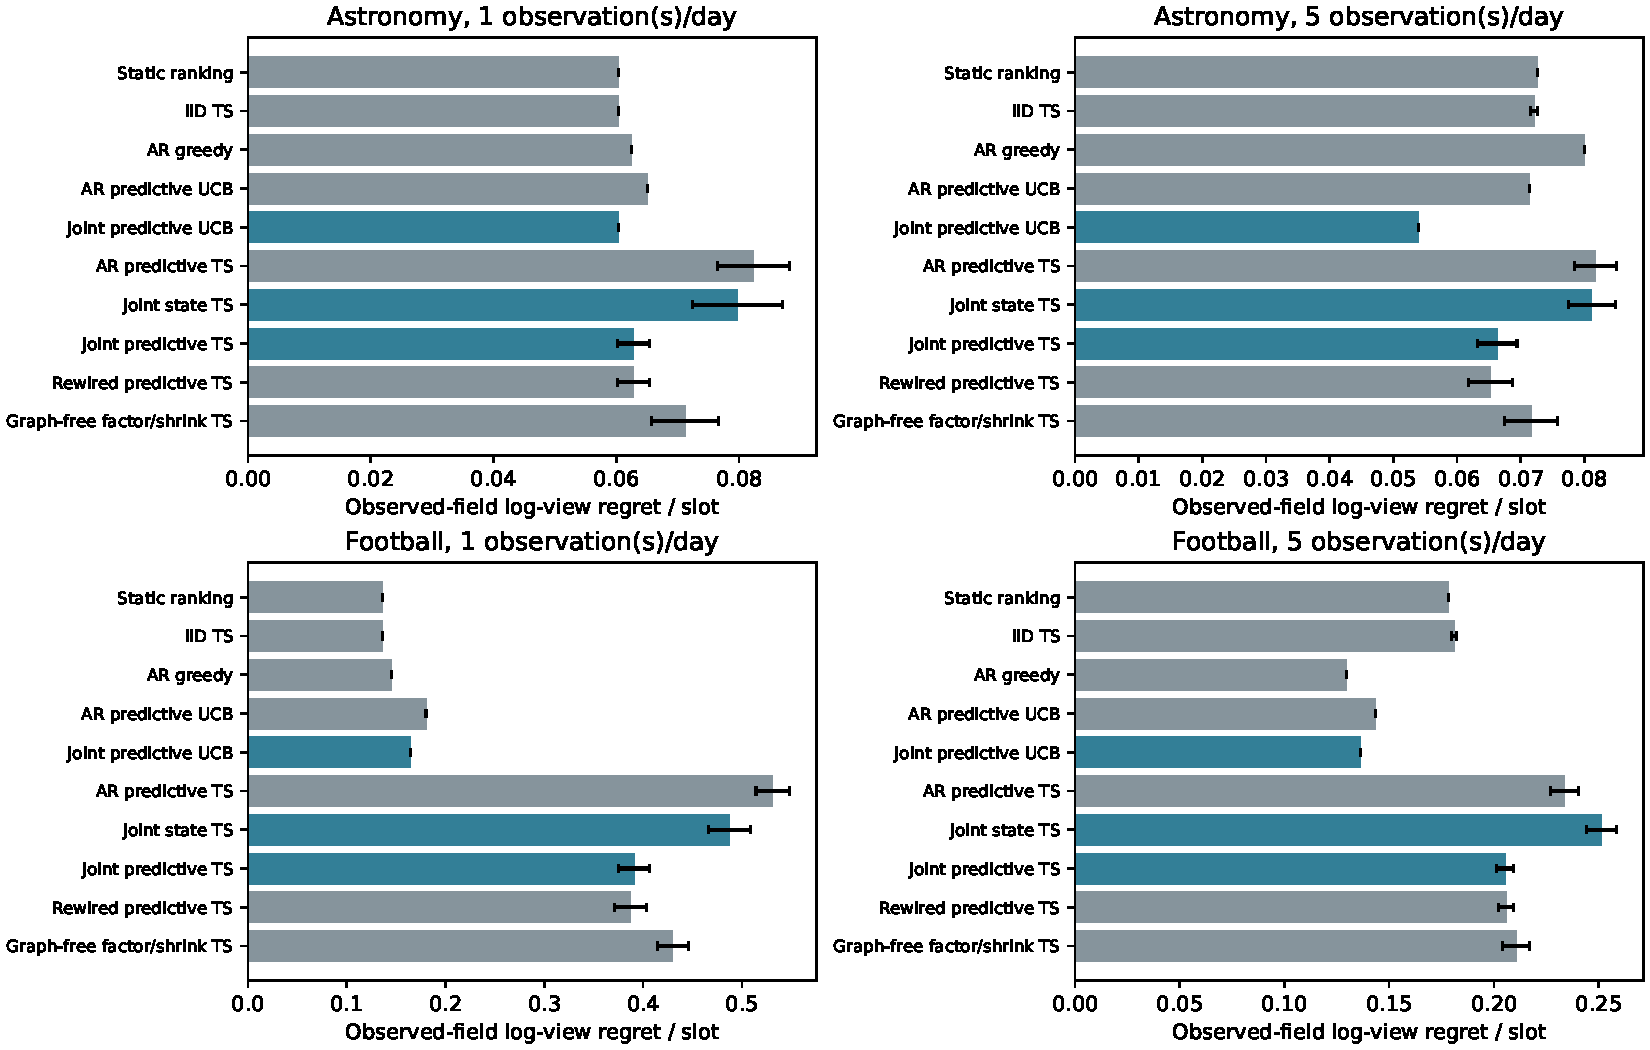
\includegraphics[width=\textwidth]{results/wikipedia/comparison.pdf}\caption{Completed Wikipedia AR(7) comparisons. Error bars are conditional 95\% Monte Carlo intervals over policy randomization on the same observed field; they are not population confidence intervals. Deterministic policies have no randomization interval.}\end{figure}

\begin{figure}[t]\centering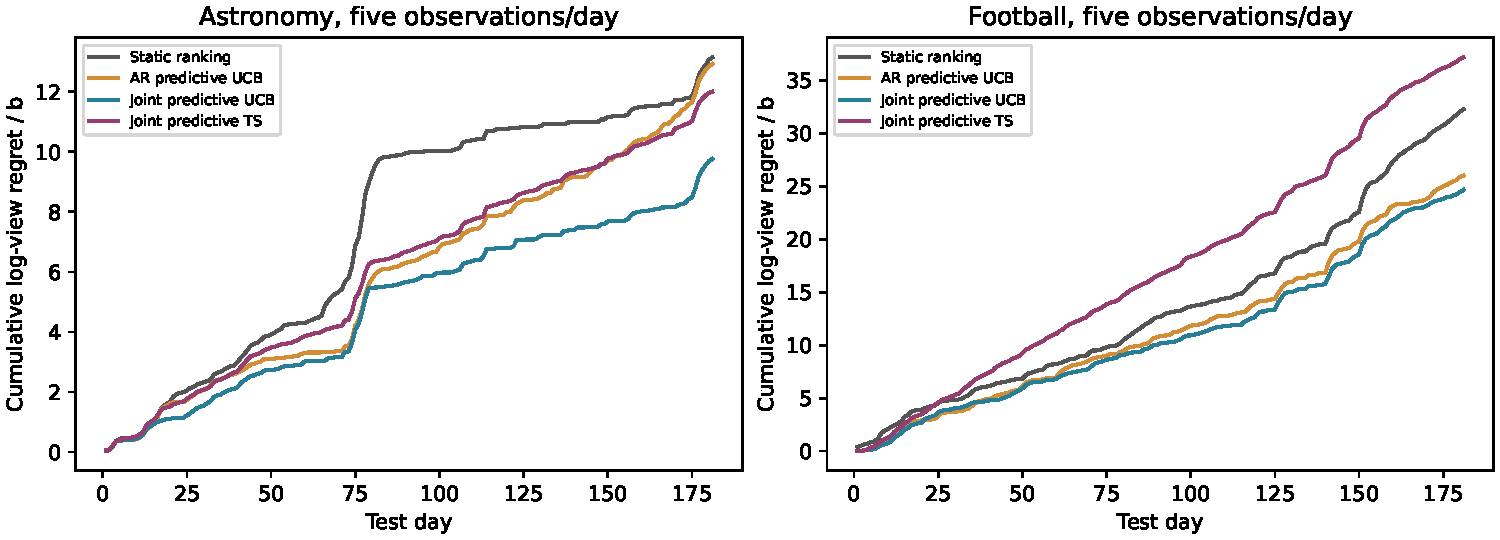
\includegraphics[width=\textwidth]{results/wikipedia/cumulative.pdf}\caption{Cumulative opportunity loss in the five-reading setting. One fixed test field per topic; no full-field test refresh is supplied to the learner.}\end{figure}

\subsection{What this application establishes}

A historical-graph, learned-general-AR selective-feedback study is feasible with a small data footprint and exact filtering. The outcomes also strengthen the negative controls: most apparent correlation benefit cannot be assigned to graph topology, and strong historical information can make simple static policies competitive. These conclusions are confined to two panels and the stated utility proxy. Raw-scale captured attention, conditional seed intervals, paired differences, monthly-block summaries, action traces and all fitted matrices are released; no theoretical floor or true stationary PCS is claimed for this real panel.
